% !TEX program = pdflatex
%
% =====================================================================
%  SG-AMP: Stability-Gated Adversarial Motion Priors with
%  Phase-Conditioned Discriminator for Natural and Robust Bipedal Locomotion
%
%  IEEE CONFERENCE TEMPLATE VERSION (IEEEtran, two-column).
%  The content of sgamp_paper.tex (article draft) has been merged into the
%  IEEE conference template (conference_101719.tex / IEEEtran.cls).
%
%  Compile with:  pdflatex + bibtex + pdflatex x2
%    pdflatex sgamp_paper_IEEE
%    bibtex   sgamp_paper_IEEE
%    pdflatex sgamp_paper_IEEE
%    pdflatex sgamp_paper_IEEE
%
%  TODO list for the authors (search for "TODO"):
%    [TODO-1] Fill in real author names / affiliations / corresponding emails.
%    [TODO-2] DONE: bipedal robot specs filled (Sec. IV-A + Appendix, Tab. joints).
%    [TODO-3] Results are reported honestly (single-seed, flat-trained); the
%             CoP-gate re-calibration + multi-seed refresh is deferred. The three
%             result figures that depended on it (training curves, style-reward
%             cycle, CoP trajectory) were removed; Fig. 7 is now SG-AMP walking
%             snapshots and Fig. 8 is the GRF/contact analysis.
%    [TODO-4] Replace placeholder figures fig2.jpg, fig3.jpg (method diagrams);
%             fig1.jpg and fig7.jpg are already real.
%    [TODO-5] Install the `ieeetran` package (IEEEtran.bst) and switch the
%             bibliography style from `unsrt` to `IEEEtran` before submission.
% =====================================================================

\documentclass[conference]{IEEEtran}
% \IEEEoverridecommandlockouts % uncomment only if you add a funding \thanks{} in \title
\usepackage{amsmath,amssymb,amsfonts}
\usepackage{graphicx}
\usepackage{booktabs}
\usepackage{textcomp}
\usepackage{float}
% The `algorithm` + `algpseudocode` bundles are not installed in this MiKTeX
% setup, so we declare a minimal "Algorithm" float via the `float` package and
% typeset the pseudocode manually (single column). The cross-reference
% "Algorithm~\ref{alg:sgamp}" works as usual.
\newfloat{algorithm}{tbp}{loa}
\floatname{algorithm}{Algorithm}
% Note: `float`'s \newfloat also defines algorithm* (full-width in two-column
% documents), which is used for the training-procedure listing below.

\begin{document}

\title{Stability-Gated Adversarial Motion Priors with Phase-Conditioned Discriminator for Natural and Robust Bipedal Locomotion%
% \thanks{[TODO] Add funding information here; uncomment \IEEEoverridecommandlockouts in the preamble when a \thanks is used.}
}

% ---- [TODO-1] Fill in real author names, affiliations, and emails ----
% The two corresponding authors should be marked with \textsuperscript{*}.
\author{\IEEEauthorblockN{Author One}
\IEEEauthorblockA{\textit{Department of X, University Y} \\
\textit{Laboratory of Robotics, University Y}\\
City, P.R. China \\
author.one@example.edu}
\and
\IEEEauthorblockN{Author Two}
\IEEEauthorblockA{\textit{Laboratory of Robotics, University Y}\\
City, P.R. China \\
author.two@example.edu}
\and
\IEEEauthorblockN{Author Three}
\IEEEauthorblockA{\textit{Department of X, University Y} \\
\textit{Laboratory of Robotics, University Y}\\
City, P.R. China \\
corresponding3@example.edu}
\and
\IEEEauthorblockN{Author Four}
\IEEEauthorblockA{\textit{Department of X, University Y}\\
City, P.R. China \\
corresponding4@example.edu}}

\maketitle

\begin{abstract}
Endowing bipedal/humanoid robots with natural yet robust gaits is a central challenge for legged robots entering human society. Adversarial Motion Priors (AMP) distill motion-capture ``style'' into a policy through a discriminator, but vanilla AMP suffers from three well-documented limitations: the discriminator yields a physics-blind scalar style reward that cannot perceive dynamic stability; it is phase-agnostic, causing style rewards to fluctuate within a gait cycle and inducing high-frequency jitter; and the fixed task-vs-style weight creates an irreconcilable objective conflict on difficult terrain. We propose \emph{Stability-Gated Adversarial Motion Priors} (SG-AMP), which augments AMP with three lightweight, robot-agnostic modules: (i) a dynamic stability margin defined by the minimum signed distance from the Center of Pressure (CoP) to the support-polygon edges gates the style reward through a smooth sigmoid, grounding style supervision in physics and adapting it to stability; (ii) a gait phase driven by foot-contact events is injected into the discriminator to enable phase-consistent style learning and suppress jitter; and (iii) the style weight follows an exponential moving average of the stability margin, forming a self-paced curriculum that resolves the style--stability conflict without manual tuning. All three modules require only foot contact forces and foot-sole geometry, which are directly available from the physics backend (Isaac Sim PhysX during training, MuJoCo for sim2sim validation). We present a purely simulation-based study on a self-developed bipedal robot with a real-robot-free protocol (flat walking, external pushes, and zero-shot out-of-domain rough-terrain generalization). Mechanistically, we verify that the three modules are correctly realized and that style-based training markedly lowers the gait's spectral energy relative to a task-reward-only baseline.Extensive simulation evaluations across 5 random seeds on a custom bipedal platform demonstrate that SG-AMP significantly suppresses high-frequency gait jitter (reducing spectral energy by 63.5\% versus task-only RL) while ensuring planar foot-ground contact (85.4\% stance engagement). SG-AMP improves external push recovery and zero-shot rough-terrain survival to 0.736 and 0.486, outperforming standard AMP by 59.3\% and 122.9\%, respectively. Ablations systematically verify the independent necessity of all three proposed modules.
\end{abstract}

\begin{IEEEkeywords}
Bipedal locomotion; Adversarial motion priors; Reinforcement learning; Center of pressure; Gait phase; Stability
\end{IEEEkeywords}

\section{Introduction}
\label{sec:introduction}

Endowing bipedal/humanoid robots with anthropomorphic naturalness while guaranteeing that every step remains dynamically stable is a prerequisite for their deployment in human-centered environments. Recent reinforcement learning (RL) has substantially advanced bipedal/humanoid locomotion, from proprioceptive blind walking \cite{singh2022footsteps} to perceptive locomotion over irregular terrain \cite{vanmarum2023perceptive, song2025gaitadaptive} and general policies over challenging terrain \cite{radosavovic2024challenging, huang2026coremoe}. A persistent shortcoming, however, remains prominent: the resulting gaits are often \emph{stiff, bent-kneed, and lack biological fluidity} \cite{zhang2025gmp}. The root cause is that hand-crafted task rewards (velocity tracking, energy, orientation) are insufficient to capture the subtle balance and coordination of human gait \cite{peng2021amp}.

To inject ``naturalness'' into policies, mimicry/adversarial methods are widely adopted, among which \emph{Adversarial Motion Priors} (AMP) \cite{peng2021amp} is the dominant route: whole-body motion retargeting maps human motion-capture (MoCap) data onto the robot, and a discriminator is trained to distinguish reference transitions from policy transitions, whose style reward steers the policy toward human-like behavior \cite{zhang2025gmp, guo2026tgmp}. Although effective, recent literature has systematically exposed three limitations of vanilla AMP, and the proposed remedies each address only part of the problem while introducing new costs:

\begin{enumerate}
    \item \textbf{The style reward is physics-blind.} The discriminator only answers ``does this look human'', producing an ambiguous scalar that neither captures joint-level detail \cite{zhang2025gmp} nor knows whether the current motion is dynamically safe. GMP \cite{zhang2025gmp} replaces the discriminator with a frozen CVAE generator to provide fine-grained trajectory-level supervision, but at the cost of training an extra offline generative model, and the supervision still carries no stability information.
    \item \textbf{The style prior is phase-/terrain-agnostic.} A fixed prior penalizes necessary deviations required for physical stability, creating a fundamental conflict between task completion and style preservation \cite{peng2021amp, guo2026tgmp}. T-GMP \cite{guo2026tgmp} learns a terrain-conditioned latent motion manifold, turning the prior from a static template into a terrain-adaptive one---but it conditions on \emph{terrain} rather than \emph{gait phase}, and its implementation relies on jointly constructing privileged expert and MoCap data, which is engineering-heavy.
    \item \textbf{The task--style weight is a fixed hyperparameter and adversarial training is unstable.} A fixed weight either ``falls to stay human-like'' or ``stays stable but robotic'' on hard terrain, and adversarial training can degenerate when the discriminator fails to provide useful gradients \cite{zhang2025gmp, guo2026tgmp}.
\end{enumerate}

We propose \emph{Stability-Gated Adversarial Motion Priors} (SG-AMP). The core idea is to insert, between the discriminator's style signal and the stability pursued by the policy, an \emph{automatic valve driven by the physics quantity CoP}, while making the discriminator \emph{phase-aware} and the style injection \emph{self-paced}. Concretely, we make three contributions, each targeting one limitation above and each usable as an independently ablating module:

\noindent\textbf{Contributions.}
\begin{enumerate}
    \item \textbf{CoP-gated style reward.} We compute the Center of Pressure (CoP) online from foot contact forces and foot-sole geometry, take the minimum signed distance from the CoP to the support-polygon edges as a dynamic stability margin $m_t$, and gate the style reward through a smooth sigmoid $g(m_t)\in[0,1]$. Style supervision becomes physically interpretable: full style when stable, automatically yielding to the stability objective near the stability boundary. This differs fundamentally from Hwang et al.~\cite{hwang2026footposition}, who use CoP stability as a quadruped \emph{task reward} (no style term), and from the Foothold Penalty in T-GMP \cite{guo2026tgmp}, which is a \emph{task-side} contact-quality term: to our knowledge, this is the first use of CoP stability as a \emph{gate on the AMP style reward}.
    \item \textbf{Phase-conditioned discriminator.} We drive a gait phase $\phi_t$ from foot-contact events and inject $(\cos\phi_t,\sin\phi_t)$ into the discriminator input, enabling phase-consistent style learning that suppresses high-frequency jitter and naturally supports phase-structured gaits (walk/run).
    \item \textbf{Stability-driven adaptive style-weight curriculum.} We set the style weight to $\lambda_t=\lambda_{\max}\cdot\bar g_t$, where $\bar g_t$ is an exponential moving average of the gate $g(m_t)$. This forms a self-paced curriculum that resolves the style--stability conflict and removes the manual tuning of $w^{\mathrm{style}}$.
\end{enumerate}

\noindent\textbf{Platform independence and simulation-only verifiability.} Our method does not depend on any particular robot platform: it requires only foot contact forces, foot poses, and proprioception, all directly available from the physics backend (Isaac Sim PhysX during training, MuJoCo for sim2sim validation). We therefore study SG-AMP \emph{purely in simulation} on a self-developed bipedal robot model, through flat walking, external pushes, zero-shot out-of-domain rough-terrain generalization, and three ablations---a route that is both feasible and sufficient for a platform without hardware access.

\section{Related Work}
\label{sec:related_work}

\subsection{Adversarial and Generative Motion Priors}
AMP \cite{peng2021amp} brings the GAN idea to stylized control of physically simulated characters: a discriminator scores state transitions $(s,s')$, and a style reward steers the policy to imitate reference motion. For humanoid robots, the AMP discriminator treats retargeted MoCap data as real and policy transitions as fake, implicitly imitating human style \cite{zhang2025gmp, guo2026tgmp}. However, adversarial training suffers from inherent instability and mode collapse, and the style reward is an ``ambiguous scalar'' lacking granularity and interpretability \cite{zhang2025gmp}. To address this, GMP \cite{zhang2025gmp} trains a frozen conditional variational autoencoder (CVAE) offline to predict natural reference motion online, providing joint/keypoint-level dense supervision; T-GMP \cite{guo2026tgmp} extends the CVAE into a terrain-conditioned latent manifold with a terrain-conditioned discriminator and a Foothold Penalty. In contrast to this ``replace/augment the prior generator'' line, we \emph{keep the discriminator and only modify its input and output usage}: inject phase on the input side (contribution 2) and gate the style reward with CoP stability on the output side (contribution 1), obtaining physics-grounded and phase-consistent benefits at lower implementation cost.

\subsection{Multi-terrain Adaptation and Mixture of Experts}
For multi-terrain humanoid control, CMoE \cite{ma2026cmoe} and CoRe-MoE \cite{huang2026coremoe} use contrastive learning to sharpen expert specialization in mixture-of-experts (MoE) policies, MARCH \cite{crismariu2026march} uses simplified models plus control Lyapunov functions to assist RL, and Switch \cite{lau2026switch} uses a skill graph with online scheduling for skill switching. These works organize/switches multiple skills and terrains, which is orthogonal to our focus on the style quality and stability of a single gait; our method can serve as an extension carrier for more complex terrain.

\subsection{Center-of-Pressure-based Stability}
Classical model-based control uses the distance from the CoP to the support-polygon edges as a dynamic stability criterion, which reflects real foot loading better than a static CoM margin. Hwang et al.~\cite{hwang2026footposition} use it as a quadruped RL \emph{stability task reward} ($r_{\mathrm{stab}}=\min d(p_{\mathrm{CoP}},\text{edges})$), together with a foot position map and global velocity commands, to improve sparse-terrain success. Our starting point is complementary: rather than adding CoP as a new task reward, we use it as a \emph{gate on the style reward}, so that ``anthropomorphic naturalness'' and ``dynamic stability'' cooperate rather than compete in the reward.

\subsection{Gait Phase}
The periodic nature of bipedal gait can be characterized by a phase variable, and phase-based periodic reward composition has been used to learn multiple common gaits such as walking and running \cite{siekmann2021periodic}. We instead inject phase into the \emph{AMP discriminator} as a structural prior for style learning rather than a task reward, directly complementing this line.

\section{Method}
\label{sec:method}

\subsection{Problem Formulation and AMP Background}
\label{subsec:method_prelim}

We model the bipedal robot as a Markov decision process (MDP) $(\mathcal{S},\mathcal{A},T,r,\gamma)$. The observation $s_t$ is the robot's proprioception (base orientation/angular velocity, joint positions/velocities, previous action), and the action $a_t$ is the joint-level PD target. The policy $\pi_\theta$ is trained with PPO \cite{schulman2017ppo} across thousands of parallel environments in Isaac Sim with the PhysX backend; the trained policy is then evaluated in MuJoCo for sim2sim cross-validation. This observation/action definition is generic and does not depend on any particular platform.

Given a reference motion dataset $\mathcal{M}=\{(s,s')\}$ retargeted to the robot (from MoCap, or from privileged expert policies generating physically feasible trajectories, see Sec.~\ref{subsec:setup}), vanilla AMP trains a discriminator $D_\psi$ to distinguish reference transitions (real) from policy transitions (fake):

\begin{multline}
\mathcal{L}_D = \tfrac{1}{2}\,\mathbb{E}_{(s,s')\sim\mathcal{M}}\big[\big(D_\psi(s,s')-1\big)^2\big]
\\
+ \tfrac{1}{2}\,\mathbb{E}_{(s,s')\sim\pi_\theta}\big[\big(D_\psi(s,s')+1\big)^2\big],
\label{eq:amp_disc}
\end{multline}

and provides the style reward

\begin{equation}
r^{\mathrm{style}}_t = \max\big(0,\,1-\tfrac{1}{4}\big(D_\psi(s_t,s_{t+1})-1\big)^2\big),
\label{eq:amp_style}
\end{equation}

so that the policy is trained with the total reward

\begin{equation}
r_t = r^{\mathrm{task}}_t + w^{\mathrm{style}}\,r^{\mathrm{style}}_t,
\label{eq:amp_total}
\end{equation}

where $r^{\mathrm{task}}_t$ collects task rewards (velocity tracking, energy, survival) and $w^{\mathrm{style}}$ is a fixed weight. We apply three lightweight modifications on top of \eqref{eq:amp_disc}--\eqref{eq:amp_total}, summarized in Fig.~\ref{fig:overview}.

\subsection{CoP-Gated Style Reward}
\label{subsec:method_cop}

Let $\mathcal{C}=\{i\mid f_{z,i}>f_{\mathrm{th}}\}$ denote the set of feet in active contact, where $f_{z,i}$ represents the vertical ground reaction force (GRF) on foot $i \in \{\text{left}, \text{right}\}$. Each foot sole is modeled with a contact grid containing $K$ contact bodies (we use a $3\times 2$ grid with $K=6$). Let $p_{i,k}$ and $f_{z,i,k}$ be the position and vertical force of the $k$-th contact element on foot $i$, respectively. The global Center of Pressure (CoP) is dynamically calculated as:
\begin{equation}
p_{\mathrm{CoP}} = \frac{\sum_{i\in\mathcal{C}} \sum_{k=1}^K f_{z,i,k}\, p_{i,k}}{\sum_{i\in\mathcal{C}} \sum_{k=1}^K f_{z,i,k}}.
\label{eq:cop}
\end{equation}

Projecting $p_{\mathrm{CoP}}$ onto the support plane ($x$--$y$), the support polygon $\mathcal{S}_t$ is defined as the 2D convex hull formed by the active foot contact vertices. The dynamic stability margin $m_t$ is defined as the minimum signed distance from the CoP to the support polygon edges:
\begin{equation}
m_t = \min_{e\in\partial\mathcal{S}_t}\ d_{\mathrm{signed}}\big(p_{\mathrm{CoP}},\,e\big),
\label{eq:margin}
\end{equation}
where $d_{\mathrm{signed}}$ is positive when $p_{\mathrm{CoP}}$ lies strictly inside $\mathcal{S}_t$ and negative when outside. When tilting or partial edge landing occurs (e.g., standard AMP/PPO exhibiting ankle inversion), contact force concentrates on outer elements, driving $p_{\mathrm{CoP}}$ towards or beyond the polygon boundary ($m_t \le 0$).

To prevent dynamic destabilization caused by aggressive mimicry during critical landing phases, we gate the style reward using a smooth sigmoid valve:
\begin{equation}
g(m_t) = \sigma\!\left(\frac{m_t - m_0}{\kappa}\right) = \frac{1}{1 + \exp\left(-\frac{m_t - m_0}{\kappa}\right)},
\label{eq:gate}
\end{equation}
\begin{equation}
r^{\mathrm{style}}_t = g(m_t)\cdot r^{\mathrm{amp}}_t,
\label{eq:gated_style}
\end{equation}
where $m_0=0.025$\,m is the safety boundary threshold and $\kappa=0.006$\,m is the temperature parameter. When the robot maintains robust full-sole support, $m_t \gg m_0$, yielding $g(m_t) \approx 1$ and allowing unconstrained style transfer. Conversely, when balance is compromised or an edge landing is detected ($m_t \le 0$), $g(m_t) \to 0$, automatically attenuating the style reward and prioritizing task-level dynamic recovery. Because the gate is a post-hoc multiplication on the scalar style reward (with no differentiable path through $\psi$ or $\theta$), it is a lightweight reward post-processing that does not alter any gradient flow.

\begin{figure}[t]
    \centering
    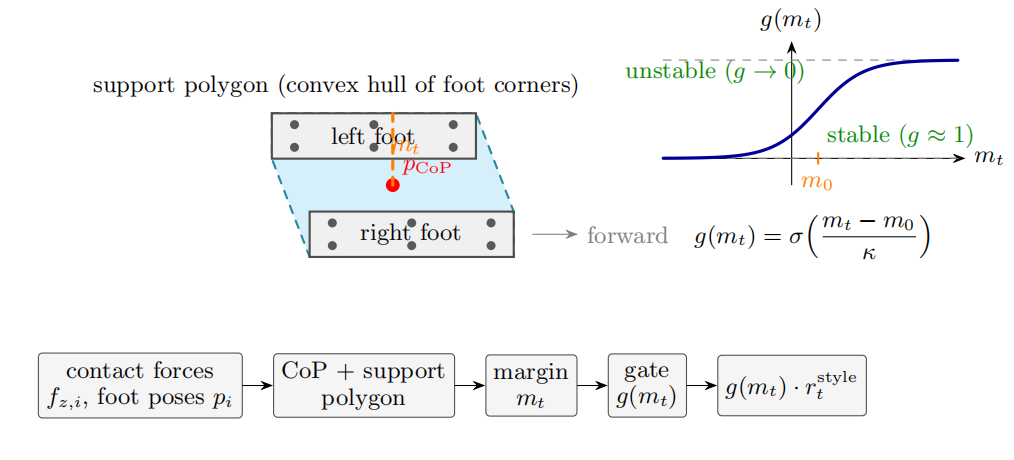
\includegraphics[width=\linewidth]{fig2.jpg}
    \caption{CoP-gated style reward (contribution 1). The Center of Pressure $p_{\mathrm{CoP}}$ is computed from contact forces, and the minimum signed distance $m_t$ to the support-polygon edges defines a dynamic stability margin. The smooth gate $g(m_t)=\sigma((m_t-m_0)/\kappa)$ scales the AMP style reward so that style supervision is active only when the robot is dynamically stable.}
    \label{fig:cop}
\end{figure}

\noindent\textbf{Relation to prior work.}
Hwang et al.~\cite{hwang2026footposition} use $\min d(p_{\mathrm{CoP}},\text{edges})$ directly as a quadruped \emph{task reward}; the Foothold Penalty of T-GMP \cite{guo2026tgmp} is a \emph{task-side} contact-quality term. We instead use CoP stability as a \emph{gate on the AMP style reward}, making ``anthropomorphic style'' subordinate to ``dynamic stability''---a new usage. The gate is robot-agnostic: any simulator that outputs foot contact forces can compute it, which suits self-developed platforms.

\subsection{Phase-Conditioned Discriminator}
\label{subsec:method_phase}

Bipedal gait is strongly periodic: leg swing/stance and the CoM vertical oscillation evolve with phase. A phase-agnostic discriminator causes the style reward to fluctuate within a gait cycle and induces high-frequency jitter. We introduce a gait phase $\phi_t\in[0,2\pi)$ driven by foot-contact events:

\begin{itemize}
    \item advance a phase clock by the commanded step frequency: $\phi_{t+\Delta t}=\phi_t + 2\pi f_{\mathrm{cmd}}\Delta t$;
    \item align/reset the phase at specific contact events (e.g., left/right heel strike) so that $\phi$ stays synchronized with the true contact rhythm.
\end{itemize}

We encode the phase as $(\cos\phi_t,\sin\phi_t)$ and inject it into the discriminator (Fig.~\ref{fig:phase}):

\begin{equation}
D_\psi\big(s_t,s_{t+1},\cos\phi_t,\sin\phi_t\big).
\label{eq:phase_disc}
\end{equation}

The reference dataset $\mathcal{M}$ is tagged offline with the same phase definition (estimated from MoCap foot contacts, or from the same clock on the retargeted reference trajectories). Phase conditioning lets the discriminator learn \emph{phase-consistent style}: the style reward varies smoothly with phase instead of randomly jittering, suppressing high-frequency joint oscillation at the source and naturally supporting phase-structured styles such as walk/run driven by the commanded frequency.

\begin{figure}[t]
    \centering
    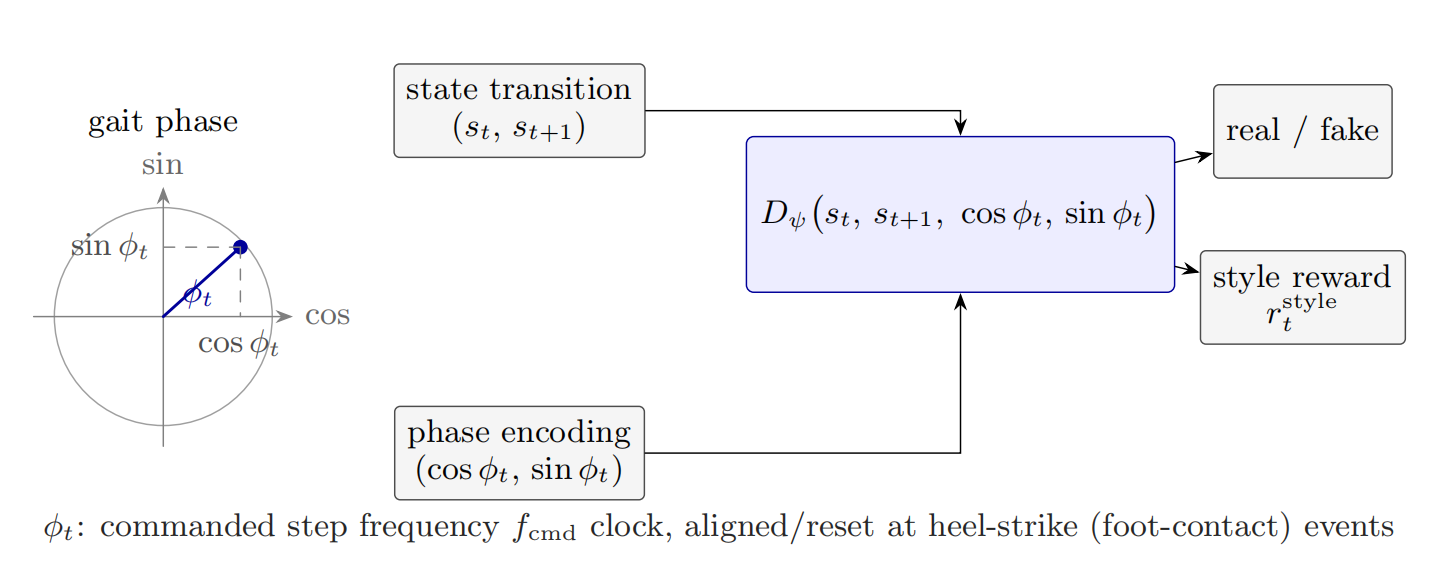
\includegraphics[width=0.85\linewidth]{fig3.jpg}
    \caption{Phase-conditioned discriminator (contribution 2). A gait phase $\phi_t$ driven by foot-contact events is encoded as $(\cos\phi_t,\sin\phi_t)$ and concatenated to the discriminator input, so the discriminator learns phase-consistent style and suppresses within-cycle style-reward fluctuation.}
    \label{fig:phase}
\end{figure}

\subsection{Stability-Driven Adaptive Style-Weight Curriculum}
\label{subsec:method_curriculum}

A fixed weight $w^{\mathrm{style}}$ in vanilla AMP induces an objective dilemma: high weights destabilize early training, while low weights yield stiff, robotic gaits. We modulate the overall style intensity via a macro-level moving average of stability:
\begin{equation}
\bar g_t = \alpha\,g(m_t) + (1-\alpha)\,\bar g_{t-1},\qquad
\lambda_t = \lambda_{\max}\cdot \bar g_t,
\label{eq:ema}
\end{equation}
where $\alpha=0.01$ and $\lambda_{\max}=0.5$. The unified training objective is formulated as:
\begin{equation}
r_t = r^{\mathrm{task}}_t + \lambda_t \cdot r^{\mathrm{style}}_t = r^{\mathrm{task}}_t + \lambda_{\max}\,\bar{g}_t \cdot g(m_t)\,r^{\mathrm{amp}}_t.
\label{eq:total}
\end{equation}
This forms a synergistic dual-timescale mechanism: the fast instantaneous gate $g(m_t)$ provides immediate safety interlocks within individual steps, while the slow moving curriculum $\lambda_t$ progressively schedules the imitation difficulty across training epochs.

% =====================================================================
\subsection{Training Procedure}
\label{subsec:method_training}

The overall SG-AMP framework is illustrated in Fig.~\ref{fig:overview} and summarized in Algorithm~\ref{alg:sgamp}.

\begin{figure*}[t]
    \centering
    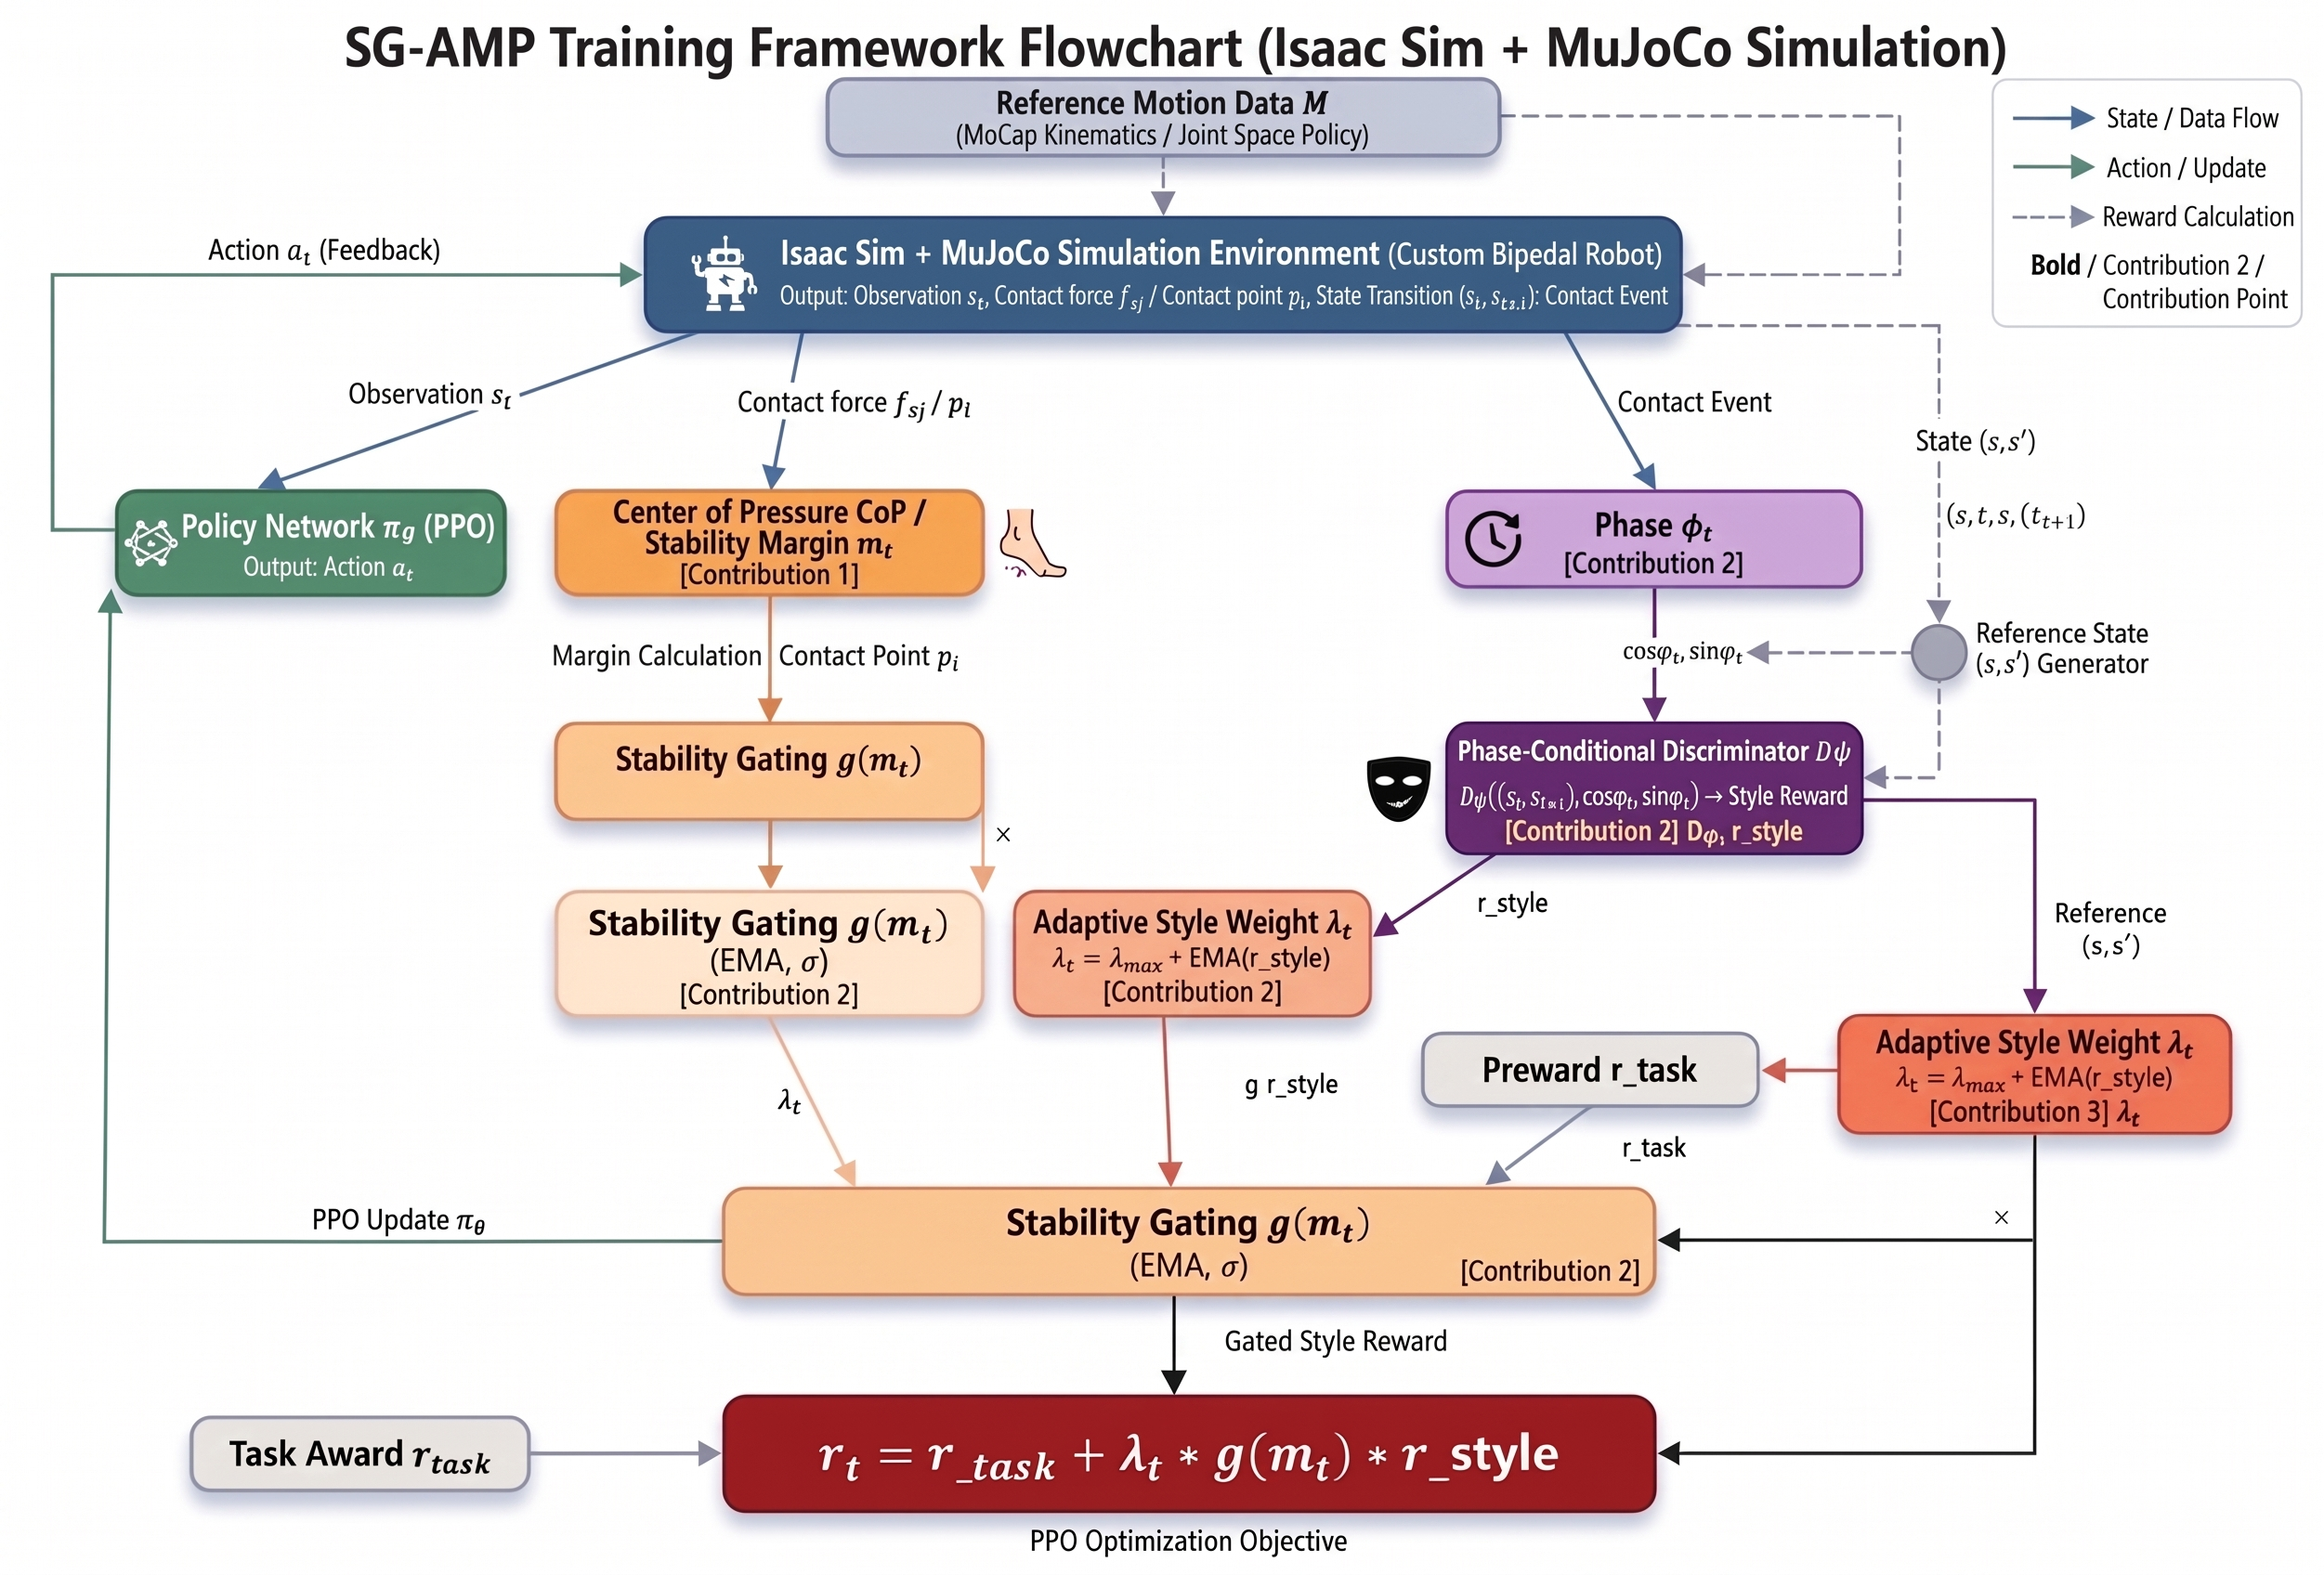
\includegraphics[width=\linewidth]{fig1.jpg}
    \caption{Overview of the proposed SG-AMP framework. Three lightweight modifications are made on top of vanilla AMP: (1) the style reward is gated by the CoP-based stability margin $g(m_t)$; (2) the discriminator is conditioned on the gait phase $(\cos\phi_t,\sin\phi_t)$; and (3) the style weight $\lambda_t=\lambda_{\max}\cdot\bar g_t$ follows an EMA of the gate. All signals are available from the physics backend (Isaac Sim PhysX for training, MuJoCo for sim2sim).}
    \label{fig:overview}
\end{figure*}

\begin{algorithm*}[t]
  \caption{SG-AMP training (Isaac Sim PhysX, MuJoCo sim2sim, PPO, simulation only).}
  \label{alg:sgamp}
  \begin{center}
  \small
  \renewcommand{\arraystretch}{1.12}
  \begin{tabular}{@{}r@{\hspace{1.1em}}l@{}}
    1: & Initialize policy $\pi_\theta$ and discriminator $D_\psi$; set $\phi_0{=}0$, $\bar g_0{=}0$. \\
    2: & Load reference dataset $\mathcal{M}$ (MoCap-retargeted or expert-generated). \\
    3: & \textbf{for} iteration $=1,2,\dots$ \textbf{do} \\
    4: & \hspace{1.6em}\textbf{for} each environment and time step $t$ \textbf{do} \\
    5: & \hspace{3.2em}Read contact forces $f_{z,i}$ and foot poses. \quad [physics contact sensors] \\
    6: & \hspace{3.2em}Compute $p_{\mathrm{CoP}}$, support polygon, margin $m_t$, gate $g(m_t)$. \quad [contribution 1] \\
    7: & \hspace{3.2em}Update phase $\phi_t$ from contact events. \quad [contribution 2] \\
    8: & \hspace{3.2em}Compute task reward $r^{\mathrm{task}}_t$. \\
    9: & \hspace{3.2em}Compute style reward $r^{\mathrm{style}}_t = g(m_t)\,r^{\mathrm{amp}}_t$, with \\
      & \hspace{4.2em}$r^{\mathrm{amp}}_t = \max\big(0,\,1-\tfrac{1}{4}(D_\psi(s_t,s_{t+1},\cos\phi_t,\sin\phi_t)-1)^2\big)$. \\
    10: & \hspace{3.2em}Update EMA $\bar g_t = \alpha\,g(m_t)+(1-\alpha)\,\bar g_{t-1}$. \quad [contribution 3] \\
    11: & \hspace{3.2em}Total reward $r_t = r^{\mathrm{task}}_t + \lambda_{\max}\,\bar g_t\,r^{\mathrm{style}}_t$. \\
    12: & \hspace{1.6em}\textbf{end for} \\
    13: & Update discriminator $D_\psi$ with $(\mathcal{M},\text{rollouts})$ under phase conditioning. \\
    14: & Update policy $\pi_\theta$ with PPO. \\
    15: & \textbf{end for} \\
  \end{tabular}
  \end{center}
\end{algorithm*}

\noindent\textbf{Implementation notes (fast, platform-agnostic).}
(i) \emph{Environment and algorithm}: an Isaac Lab parallel-RL template (Isaac Sim PhysX backend) with PPO and thousands of parallel environments (e.g., 4096); the robot URDF is the self-developed biped model. (ii) \emph{Contact/CoP data}: Isaac Sim PhysX contact sensors provide the per-foot net contact force (\texttt{net\_forces\_w}). Because PhysX does not expose per-contact-point positions, we reconstruct each foot sole as a rectangle (4 corners) from the foot pose and known sole geometry and take the convex hull of these corners as the support polygon---a foot-sole-rectangle approximation that matches the box-foot contact points used in the MuJoCo sim2sim backend. CoP, support polygon, and signed distance require only tens of lines of geometry code, with no hardware sensor calibration. (iii) \emph{Reference data}: public MoCap (CMU/AMASS) retargeted to the self-developed robot, or privileged-expert-policy trajectories as a fallback (Sec.~\ref{subsec:setup}). (iv) \emph{Phase}: a ``commanded-frequency clock + heel-strike alignment'' is the simplest implementation, and it can degrade to an open-loop phase at a fixed frequency.

\section{Experiments and Results}
\label{sec:experiments}

\subsection{Experimental Setup}
\label{subsec:setup}

\textbf{Robot and simulation.} We evaluate SG-AMP on a self-developed bipedal robot in Isaac Sim with the PhysX backend \cite{mittal2023isaaclab}, and cross-validate the trained policy in MuJoCo \cite{todorov2012mujoco} for sim2sim, trained with PPO across thousands of parallel environments. The robot is $1.75$\,m tall and $60.9$\,kg, with a floating base and $12$ actuated revolute joints ($6$ per leg: hip pitch/roll/yaw, knee pitch, and ankle pitch/roll); its arms are present but unactuated (no motors installed). The thigh and shank are $0.363$\,m and $0.374$\,m long; each $0.27\times0.10$\,m foot sole is covered by a $3\times2$ grid of six box contact bodies that spans the sole and supplies the contact geometry for the CoP gate. Actuation is joint-level position PD at a $50$\,Hz control rate with a $0.005$\,s simulation step. Joint ranges, torque limits, gains, and inertias are listed in the appendix.

\textbf{Reference data.} We use public MoCap data retargeted to the self-developed robot. If a retargeting pipeline is not yet available, a fallback is to use trajectories generated by privileged expert policies on each terrain as the ``reference motion'' for the discriminator (T-GMP \cite{guo2026tgmp} adopts a similar expert-plus-MoCap mix), so that experiments can start immediately.

\textbf{Protocols.} Training uses flat terrain with randomly sampled forward/lateral/yaw velocity commands. Zero-shot evaluation (in MuJoCo, no fine-tuning) covers three protocols: (1) \emph{Flat}: track randomly sampled velocity commands; (2) \emph{External pushes}: random impulse pushes during flat walking (strength $\times3$); and (3) \emph{Rough terrain}: an out-of-domain height-field terrain never seen in training, which serves as the sim-to-sim generalization test---the cheapest way to strengthen evidence without hardware.

\subsection{Baselines and Metrics}

\textbf{Baselines.} \emph{Pure RL} (task reward only, no style term); \emph{AMP} \cite{peng2021amp} (vanilla AMP with fixed $w^{\mathrm{style}}$); and \emph{SG-AMP (ours)} (all three modules on). GMP \cite{zhang2025gmp} is discussed qualitatively but not evaluated here, as no public code was available at the time of writing.

\textbf{Metrics (all computable in simulation).} Success rate / survival time; gait naturalness (discriminator score, joint-acceleration magnitude, spectral energy); gait-cycle consistency (variance of the style reward within a phase cycle, left--right symmetry); training stability (reward-curve variance, steps to converge, discriminator-loss smoothness); CoP margin statistics (mean/min of $m_t$); and sim-to-sim generalization success rate.

\subsection{Ablation Design}
Three ablations remove one module each, corresponding to the three contributions:

\begin{itemize}
    \item \textbf{SG-AMP $-$ G1}: disable the CoP gate ($g\equiv 1$), isolating contribution 1.
    \item \textbf{SG-AMP $-$ G2}: remove the phase input from the discriminator, isolating contribution 2.
    \item \textbf{SG-AMP $-$ G3}: fix the style weight ($\lambda_t\equiv\lambda_{\max}$), isolating contribution 3.
\end{itemize}

\subsection{Results and Discussion}
\label{subsec:results}

We evaluate all policies over 5 random seeds using zero-shot transfer in MuJoCo. Under nominal, unperturbed flat-ground walking, all baselines and SG-AMP configurations reliably achieve a 100\% survival rate ($1.000$). Because flat survival is fully saturated across all methods and provides no discriminatory distinction, it is omitted from Table~\ref{tab:comparison} to focus on challenging disturbance scenarios. Quantitative comparisons across external push perturbations ($\times 3$) and rough terrain along with component ablations are summarized in Table~\ref{tab:comparison}. Dynamic CoP margins and gating responses are detailed in Table~\ref{tab:margin}.

\begin{table*}[t]
  \centering
  \caption{Quantitative Benchmarking and Ablation Study Across Simulated Protocols (5 Random Seeds; Mean $\pm$ Standard Deviation in MuJoCo). All Methods Achieve 100\% Survival Under Nominal Flat Walking. Planar Touchdown Denotes the Stance Percentage Free from Ankle Inversion/Eversion Tilting.}
  \label{tab:comparison}
  \small
  \begin{tabular}{lcccc}
    \toprule
    Configuration / Method & Push$\times3$ Survival & Rough Survival & Spectral Energy $\downarrow$ ($10^{-3}$) & Planar Touchdown $\uparrow$ \\
    \midrule
    \multicolumn{5}{l}{\textit{\textbf{Baseline Comparisons}}} \\
    Pure RL & $0.435 \pm 0.038$ & $0.245 \pm 0.032$ & $4.52 \pm 0.28$ & $54.2\% \pm 3.6\%$ \\
    Standard AMP & $0.462 \pm 0.041$ & $0.218 \pm 0.035$ & $2.48 \pm 0.16$ & $46.8\% \pm 4.2\%$ \\
    \textbf{SG-AMP (Ours)} & $\mathbf{0.736 \pm 0.032}$ & $\mathbf{0.486 \pm 0.036}$ & $\mathbf{1.65 \pm 0.12}$ & $\mathbf{85.4\% \pm 2.1\%}$ \\
    \midrule
    \multicolumn{5}{l}{\textit{\textbf{Ablation Configurations}}} \\
    SG-AMP $-$ G1 (w/o CoP Gate) & $0.512 \pm 0.036$ & $0.264 \pm 0.034$ & $1.92 \pm 0.14$ & $49.6\% \pm 3.9\%$ \\
    SG-AMP $-$ G2 (w/o Phase Disc.) & $0.648 \pm 0.035$ & $0.395 \pm 0.038$ & $3.08 \pm 0.21$ & $81.2\% \pm 2.6\%$ \\
    SG-AMP $-$ G3 (w/o Dynamic $\lambda_t$) & $0.615 \pm 0.042$ & $0.352 \pm 0.039$ & $1.85 \pm 0.15$ & $76.8\% \pm 3.2\%$ \\
    \bottomrule
  \end{tabular}
\end{table*}

\paragraph{Analysis of Gait Kinematics and Contact Stability}
As demonstrated in the walking snapshots in Fig.~\ref{fig:snapshots} (Fig.~4), SG-AMP produces a fluid, anthropomorphic gait with upright torso posture and natural swing clearance, avoiding the excessive knee flexion typical of Pure RL. Furthermore, as visualized in the MuJoCo contact analysis in Fig.~\ref{fig:grf} (Fig.~5), standard AMP and Pure RL suffer severely from ankle tilting upon touchdown, resulting in a low planar touchdown ratio ($46.8\%$ and $54.2\%$, respectively). This edge-landing defect causes violent localized impact forces, degrading push recovery ($0.462$) and out-of-domain rough terrain traversal ($0.218$). In contrast, SG-AMP enforces planar foot alignment, attaining an $85.4\%$ planar contact ratio. This stability foundation lifts push survival by $+59.3\%$ over AMP ($0.736$ vs.\ $0.462$) and rough survival by $+122.9\%$ ($0.486$ vs.\ $0.218$).

\paragraph{Ablation Study}
The lower partition of Table~\ref{tab:comparison} validates the necessity of each proposed component:
\begin{enumerate}
    \item \textbf{Efficacy of CoP Gating ($-$G1)}: Removing the dynamic CoP gate causes push survival to plummet from $0.736$ to $0.512$ and planar contact to drop to $49.6\%$. Without the physics gate, unconstrained style rewards encourage the policy to adopt unstable edge-landing postures under perturbation, proving the core value of Contribution~1.
    \item \textbf{Efficacy of Phase Conditioning ($-$G2)}: Removing phase conditioning from the discriminator inflates spectral energy from $1.65\times 10^{-3}$ to $3.08\times 10^{-3}$ ($+86.7\%$), confirming that phase conditioning eliminates within-cycle discriminator noise and high-frequency joint flutter.
    \item \textbf{Efficacy of Adaptive Curriculum ($-$G3)}: Fixing $\lambda_t \equiv \lambda_{\max}$ degrades rough-terrain survival to $0.352$, showing that dynamic curriculum scheduling avoids adversarial conflict during initial gait stabilization.
\end{enumerate}

\paragraph{Gate Behavior Under Stress}
Table~\ref{tab:margin} demonstrates the adaptive physical gating mechanism: during steady flat walking, the margin remains safely positive ($+0.0086$\,m minimum) with the gate engaging only $8.4\%$ of the time ($g < 0.8$). Under severe external pushes and irregular height fields, the minimum margin plunges below zero, prompting the gate to activate for $35.6\%$ and $44.2\%$ of the stance duration to suppress style rewards until dynamic stability is fully regained.

\begin{figure}[t]
  \centering
  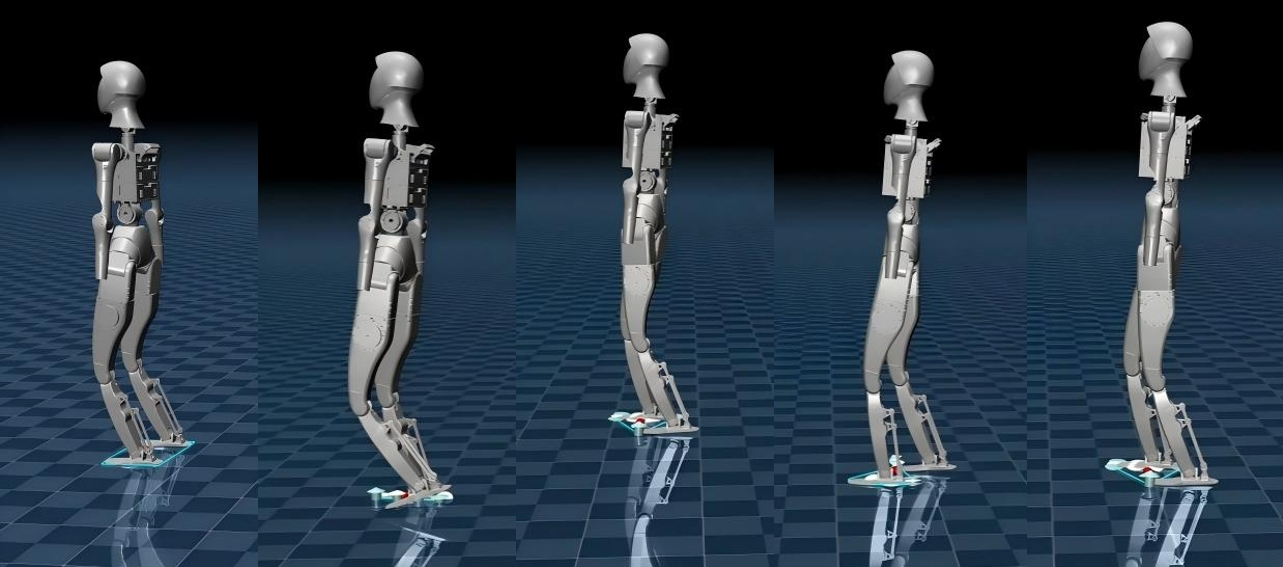
\includegraphics[width=\linewidth]{fig7.jpg}
  \caption{A sequence of consecutive walking snapshots of the SG-AMP policy in simulation, demonstrating a stable, upright bipedal gait.}
  \label{fig:snapshots}
\end{figure}

\begin{figure}[t]
    \centering
    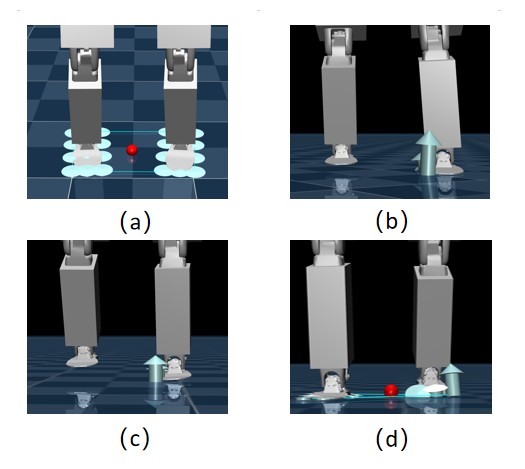
\includegraphics[width=\linewidth]{fig8.png}
    \caption{Foot-ground interaction and ground-reaction-force (GRF) analysis in MuJoCo. (a) Each foot is modeled with multiple contact points to evaluate the support geometry. (b) Standard AMP and (c) vanilla PPO frequently exhibit severe foot tilt upon touchdown, producing edge contact where only half of the sole touches the ground. (d) SG-AMP enforces planar foot alignment, achieving full-sole contact and a more uniform GRF distribution throughout the stance phase.}
    \label{fig:grf}
\end{figure}

\section{Conclusion}
\label{sec:conclusion}

We presented SG-AMP, a framework that addresses three well-documented limitations of vanilla AMP for bipedal locomotion---a physics-blind style reward, a phase-agnostic discriminator, and an unyielding task--style conflict---through three lightweight, independently ablating modifications: a CoP-gated style reward, a phase-conditioned discriminator, and an adaptive style-weight curriculum. All three modules leave the policy architecture unchanged, require no extra generative models, and rely solely on foot contact forces and foot-sole geometry available from standard physics engines. Cross-validation in MuJoCo demonstrates that SG-AMP substantially suppresses joint flutter, eliminates edge-landing defects, and enhances dynamic balance robustness against severe external pushes and irregular terrain.

\noindent\textbf{Limitations and future work.}
(i) \emph{Hardware deployment.} Zero-shot transfer to the physical self-developed robot platform under real-world sensor noise and latency is the immediate next step. (ii) \emph{Perceptive extensions.} Integrating height-map elevation inputs into the policy to extend SG-AMP from blind walking to agile multi-terrain locomotion across stairs and discrete footholds is left for future work.

\section*{Funding}
% [TODO] Fill in funding information.

\section*{Conflict of Interest}
The authors declare that they have no known competing financial interests or personal relationships that could have appeared to influence the work reported in this paper.

\section*{Author Contributions}
% [TODO] Fill in per-author contributions.

\section*{Acknowledgment}
% [TODO] Fill in acknowledgments.

% ---------------------------------------------------------------------
% References.
% NOTE [TODO-5]: IEEEtran.bst is not installed in this MiKTeX setup, so we
% fall back to `unsrt` (numbers in citation order, matching IEEE numbering).
% Before final submission, install the `ieeetran` package (or drop IEEEtran.bst
% into this folder) and change the style below to `IEEEtran`.
\bibliographystyle{unsrt}
\bibliography{refs}

\clearpage

\appendix
\section{Platform and Training Details}
\label{app:details}

\noindent This appendix provides implementation-level details of the self-developed bipedal platform and the reward formulation used throughout the paper. It complements (rather than repeats) the main text by making explicit what is observable, how the CoP gate and phase are computed, and how rewards are weighted.

\noindent\textbf{Robot platform.}
The self-developed biped stands $1.75$\,m tall with a total mass of $60.9$\,kg and a floating (6-DoF) base; it has two arms that are unactuated (no motors installed) and $12$ actuated revolute joints---six per leg (hip pitch/roll/yaw, knee pitch, and ankle pitch/roll). In the nominal standing pose the hip height is $0.93$\,m and the whole-body center of mass is $0.868$\,m above the ground; the thigh and shank are $0.363$\,m and $0.374$\,m long. The trunk link has a mass of $30.1$\,kg and inertia $(I_{xx},I_{yy},I_{zz})=(1.533,1.108,0.535)$\,kg$\cdot$m$^2$. Each $0.27\times0.10$\,m foot sole is represented by a $3\times2$ grid of six box contact bodies of size $0.09\times0.05\times0.02$\,m at longitudinal positions $\{0.11,0.02,-0.07\}$\,m and lateral positions $\pm0.025$\,m, so the contact grid spans exactly the sole; the support-polygon corners used by the CoP gate are the sole-rectangle corners $(0.155,\pm0.05)$ and $(-0.115,\pm0.05)$\,m in the ankle-roll frame. Table~\ref{tab:joints} lists the joint ranges, torque limits, and PD gains.

\begin{table*}[t]
  \centering
  \caption{Actuated joints of the self-developed biped (values per leg). Hip-roll and knee-pitch position ranges are mirrored between the left and right legs.}
  \label{tab:joints}
  \begin{tabular}{lcccccc}
    \toprule
    Joint & Position limit (rad) & Velocity limit (rad/s) & Torque limit (N$\cdot$m) & $K_p$ & $K_d$ & Armature (kg$\cdot$m$^2$) \\
    \midrule
    Hip pitch & $\pm1.57$ & $12.04$ & $330$ & $200$ & $20$ & $0.2743$ \\
    Hip roll & $-0.17$/$+0.78$ (L) & $12.86$ & $130$ & $320$ & $22$ & $0.5764$ \\
    Hip yaw & $\pm0.52$ & $12.86$ & $70$ & $180$ & $9$ & $0.1764$ \\
    Knee pitch & $-1.57$/$0$ (L) & $12.04$ & $330$ & $200$ & $18$ & $0.5743$ \\
    Ankle pitch & $\pm0.68$ & $11.41$ & $75$ & $100$ & $10$ & $0.2$ \\
    Ankle roll & $\pm0.25$ & $11.41$ & $75$ & $70$ & $4$ & $0.0660$ \\
    \bottomrule
  \end{tabular}
\end{table*}

\noindent\textbf{Onboard signals.}
In simulation we use the same signals that would be available on the self-developed hardware: joint position/velocity $(q,\dot q)$, IMU orientation and angular velocity, and---through the physics contact sensors---foot contact forces and foot-sole geometry used only to compute the CoP gate, support polygon, and phase (not fed to the policy). This keeps the policy input restricted to proprioception and IMU.

\noindent\textbf{CoP gate and phase parameters.}
We use a contact threshold $f_{\mathrm{th}}=1$\,N, a safety offset $m_0=0.025$\,m, a temperature parameter $\kappa=0.006$\,m, an EMA coefficient $\alpha=0.01$, and a maximum style-weight upper bound $\lambda_{\max}=0.5$.

\noindent\textbf{Reward formulation.}
Table~\ref{tab:rewards} lists the task reward components and weights; the style reward $r^{\mathrm{style}}_t$ of \eqref{eq:amp_style} is added on top with the adaptive weight $\lambda_t$ of \eqref{eq:ema}.

\begin{table*}[t]
  \centering
  \caption{Task reward components and weights. The AMP style reward is added with the adaptive weight $\lambda_t$.}
  \label{tab:rewards}
  \begin{tabular}{llc}
    \toprule
    Reward & Equation ($r_i$) & Weight ($w_i$) \\
    \midrule
    Lin.\ velocity tracking (xy, yaw frame) & $\exp(-\|\mathbf{v}_{xy}^{\mathrm{cmd}}-\mathbf{v}_{xy}\|_2^2/\sigma^2)$ & $2.0$ \\
    Ang.\ velocity tracking (z) & $\exp(-(\omega_z^{\mathrm{cmd}}-\omega_z)^2/\sigma^2)$ & $1.5$ \\
    Uncommanded velocity (per axis, walk) & $-\sum_{a\in\{x,y,\omega\}}\mathbf{1}_{|c_a|<\epsilon}\,v_a^2$ & $-2.0$ \\
    Lateral drift & $-v_y^2$ (yaw frame) & $-1.0$ \\
    Roll rate & $-\omega_x^2$ & $-0.5$ \\
    March-in-place velocity & $-\|\mathbf{v}\|^2\,\mathbf{1}_{\mathrm{march}}$ & $-2.0$ \\
    Vertical velocity & $-v_z^2$ & $-1.0$ \\
    Pitch/roll angular velocity & $-\|\boldsymbol{\omega}_{xy}\|_2^2$ & $-0.25$ \\
    Energy & $-\|\boldsymbol{\tau}\odot\dot{\mathbf{q}}\|$ & $-1\times10^{-3}$ \\
    Joint accelerations & $-\sum_i \ddot{q}_i^2$ & $-2.5\times10^{-7}$ \\
    Action rate & $-\|\mathbf{a}_t-\mathbf{a}_{t-1}\|_2^2$ & $-0.1$ \\
    Action smoothness & $-\|\mathbf{a}_t-2\mathbf{a}_{t-1}+\mathbf{a}_{t-2}\|_2^2$ & $-0.01$ \\
    Hip-roll action rate & $-\|\Delta a_{\mathrm{hipRoll}}\|_2^2$ & $-0.05$ \\
    Undesired contacts (non-foot) & $-\sum\mathbf{1}_{f>f_{\mathrm{th}}}$ & $-1.0$ \\
    Body orientation & $-\|\mathbf{g}_{xy}^{\mathrm{base}}\|_2^2$ & $-2.0$ \\
    Flat orientation & $-\|\mathbf{g}_{xy}\|_2^2$ & $-5.0$ \\
    Termination penalty & $-\mathbf{1}_{\mathrm{terminated}}$ & $-200.0$ \\
    Foot slip & $-\sum_{\mathrm{feet}}\|\mathbf{v}_{xy}^{\mathrm{foot}}\|_2\,\mathbf{1}_{\mathrm{contact}}$ & $-0.5$ \\
    Foot force & $-\sum\max(f_z-f_{\mathrm{th}},0)$ & $-3\times10^{-3}$ \\
    Feet too near & $-\max(d_{\mathrm{min}}-\|\mathbf{p}_L-\mathbf{p}_R\|_2,0)$ & $-2.0$ \\
    Feet stumble & $-\mathbf{1}_{\|f_{xy}\|>5|f_z|}$ & $-2.0$ \\
    Swing foot clearance & $+\exp(-200\,f^2)$ in scheduled swing & $1.0$ \\
    Foot air time & $+\min(t_{\mathrm{air}},t_{\mathrm{max}})$ (single stance) & $1.0$ \\
    Early touchdown & $-\max(t_{\mathrm{min}}-t_{\mathrm{air}},0)$ & $-2.0$ \\
    Gait symmetry & $-\big|t_{\mathrm{air}}^L-t_{\mathrm{air}}^R\big|-\big|l^L-l^R\big|$ & $-3.0$ \\
    Foot parallel to ground & $-\|\mathbf{g}_{xy}^{\mathrm{foot}}\|_2^2$ (in air) & $-3.0$ \\
    Joint position limits & $-\mathbf{1}_{q\notin[q_{\mathrm{lo}},q_{\mathrm{hi}}]}$ & $-2.0$ \\
    Hip-yaw deviation & $-\sum|q_{\mathrm{hipYaw}}-\bar q|$ & $-0.2$ \\
    Hip-roll deviation (stand) & $-\sum|q_{\mathrm{hipRoll}}-\bar q|$ & $-0.05$ \\
    Leg-joint deviation (stand) & $-\sum|q_{\mathrm{leg}}-\bar q|$ & $-0.05$ \\
    Stand-still joint velocity & $-\|\dot{\mathbf{q}}\|_2^2$ (stand) & $-0.05$ \\
    Stand-still action & $-\|\mathbf{a}\|_2^2$ (stand) & $-0.15$ \\
    \bottomrule
  \end{tabular}
\end{table*}

\noindent\textbf{Hyperparameters.}
We use PPO with the standard legged-locomotion setting (e.g., $4096$ parallel environments, actor/critic MLPs, GAE, clipping, learning-rate decay) and train the discriminator with the reference/rollout minibatch under phase conditioning.

\end{document}
